\section{Background}

\subsection{Problem Description}
\begin{figure}
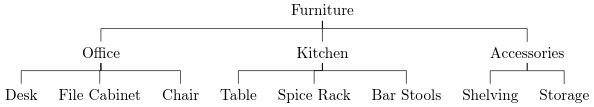
\includegraphics[width=\columnwidth]{img/hierarchy}
\caption{
Illustration of cDiscount's hierarchical classification scheme.
}
\label{fig:hierarchy}
\end{figure}

Cdiscount is one of France's largest e-commerce companies, selling everything from trampolines to televisions.
As the company grows, so does the number of different products they offer for sale.
In the past 2 years alone, they have added over 20 million new products to their catalog \cite{cDiscountKaggle}. 
The company uses a three-tier hierarchical classification system to organize its wares.
All products are assigned to a single high-level category.
This high-level categorization, such as such as ``furniture'' or ``electronics,'' is analogous to what department the product might be found in a traditional brick-and-mortar retailer. 
Within each department, products are organized into mid-level categories.
Within the high-level furniture categorization, for example, products are assigned to office, kitchen, accessories, etc. categories.
Finally, within each mid-level category, products are assigned to a single low-level category.
In the furniture department, for example, within the mid-level office categorization products are considered either a desk, a file cabinet, a chair, etc.
The categorization scheme is strictly hierarchical.
Each product belongs to a single low, mid, and high-level category; 
All products belonging to the same low-level category belong to the same mid-level category and all products belonging to the same mid-level category belong to the same high-level category.
Figure \ref{fig:hierarchy} overviews Cdiscount's product classification scheme.

Given the scale of Cdiscount's offerings, ensuring that each and every product is classified correctly is a challenging task.
Currently, Cdiscount uses machine learning text classification methods to categorize their wares.
To improve the accuracy of their classification methods, they would like to begin using images, rather than text, to categorize products.
To this end, Cdiscount sponsored a competition on the data science platform Kaggle to develop methods that automatically categorize products based on their images.
As part of this competition, they made available a data set with over 15 million images ranging over 5,000 categories.

\subsection{Data Set}

\begin{figure}
    \centering
    \begin{subfigure}[t]{0.33\columnwidth}
        \centering
        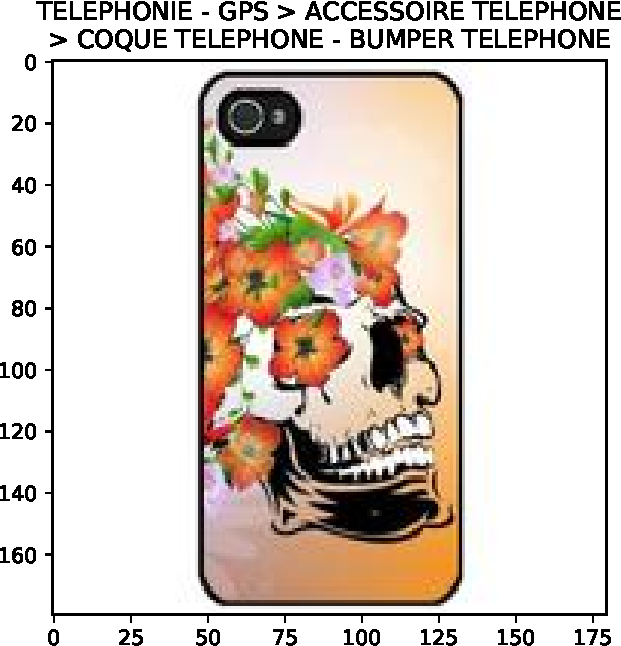
\includegraphics[width=\textwidth]{img/img-0-0}
        \caption{}
    \end{subfigure}%
    ~ 
    \begin{subfigure}[t]{0.33\columnwidth}
        \centering
        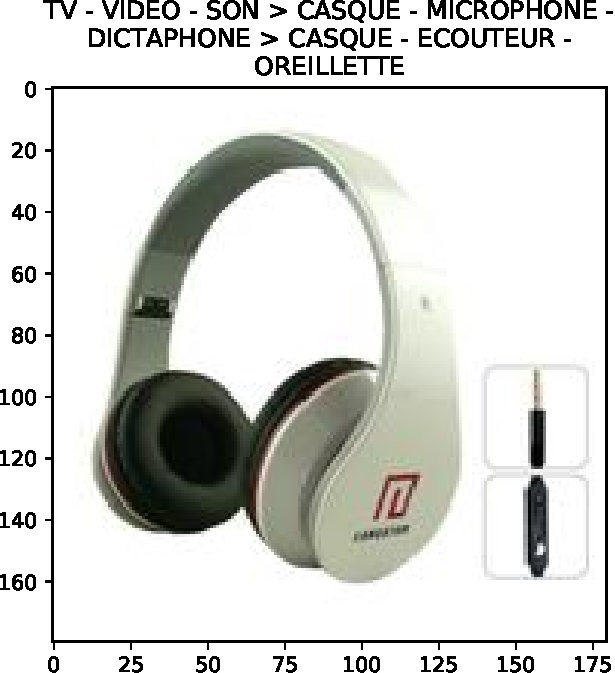
\includegraphics[width=\textwidth]{img/img-12-0}
        \caption{}
    \end{subfigure}%
    ~ 
    \begin{subfigure}[t]{0.33\columnwidth}
        \centering
        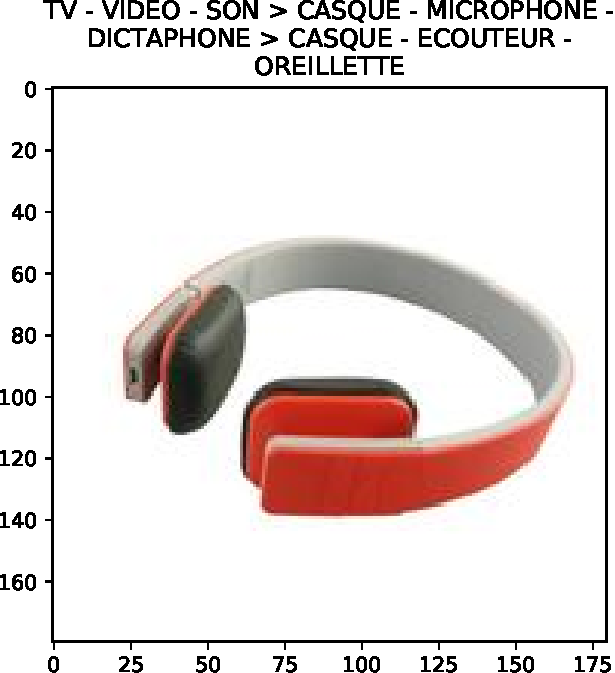
\includegraphics[width=\textwidth]{img/img-12-1}
        \caption{}
    \end{subfigure}
	\caption{
Images (a), (b), and (c) are three example training examples.
Image (a) is from a top level category different from images (b) and (c) (and therefore from different second and third categories, as well).
Images (b) and (c) are of the same product, and therefore from the same first, second, and third level categories.
Only some products, not all, have more than one associated image.
}
	\label{fig:example-images}
\end{figure}
\begin{figure}

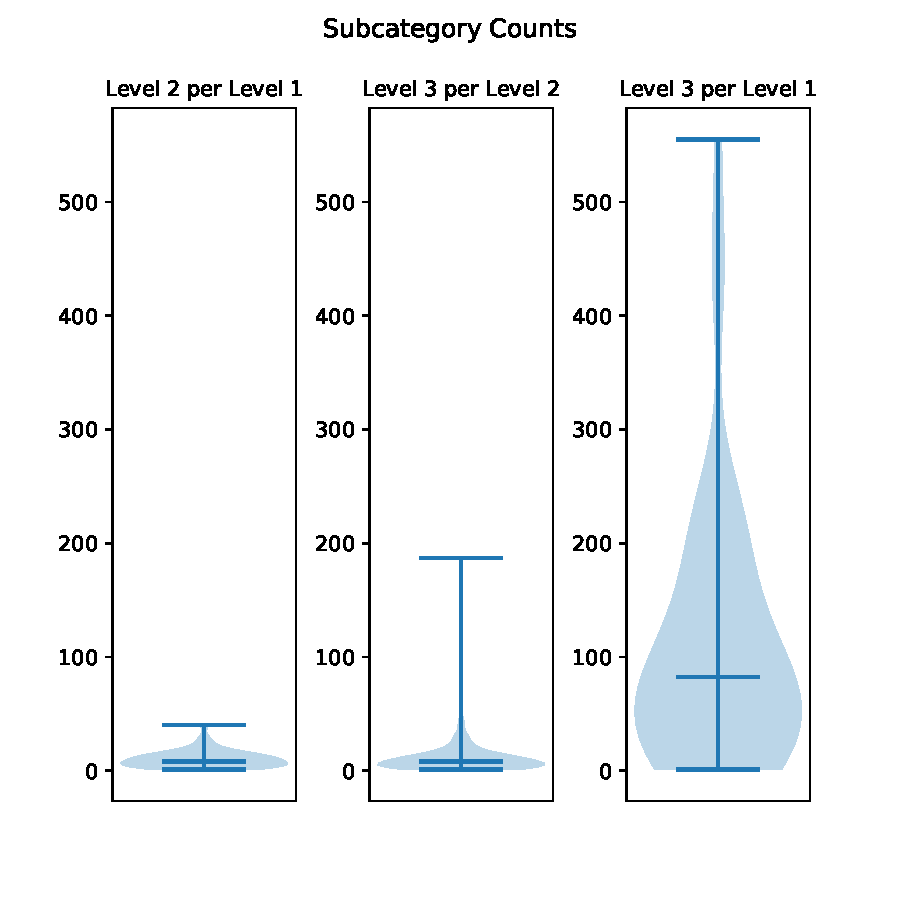
\includegraphics[width=\columnwidth]{img/catcount}
\caption{
This violin plot compares hierarchical category branching in the Cdiscount dataset.
The leftmost subplot presents the distribution of the number of second level subcategories in each top-level category.
The middle subplot presents the distribution of the number of third (bottom) level subcategories in each second level category.
The rightmost subplot presents the distribution of the number of bottom level subcategories in each first level category.
Going from first to second level and second to third level, categories branch by a median factor of approximately 10. 
From first to third level, categories branch by a median factor of approximately 100.
All three branching factor distributions have long right tails.
For example, going from second to third level, some categories are observed to branch by a factor of more than 150.
In all three subplots, horizontal bars mark the 0, 50, and 100th percentile counts.
}
\label{fig:catcount}

\end{figure}
\begin{figure}
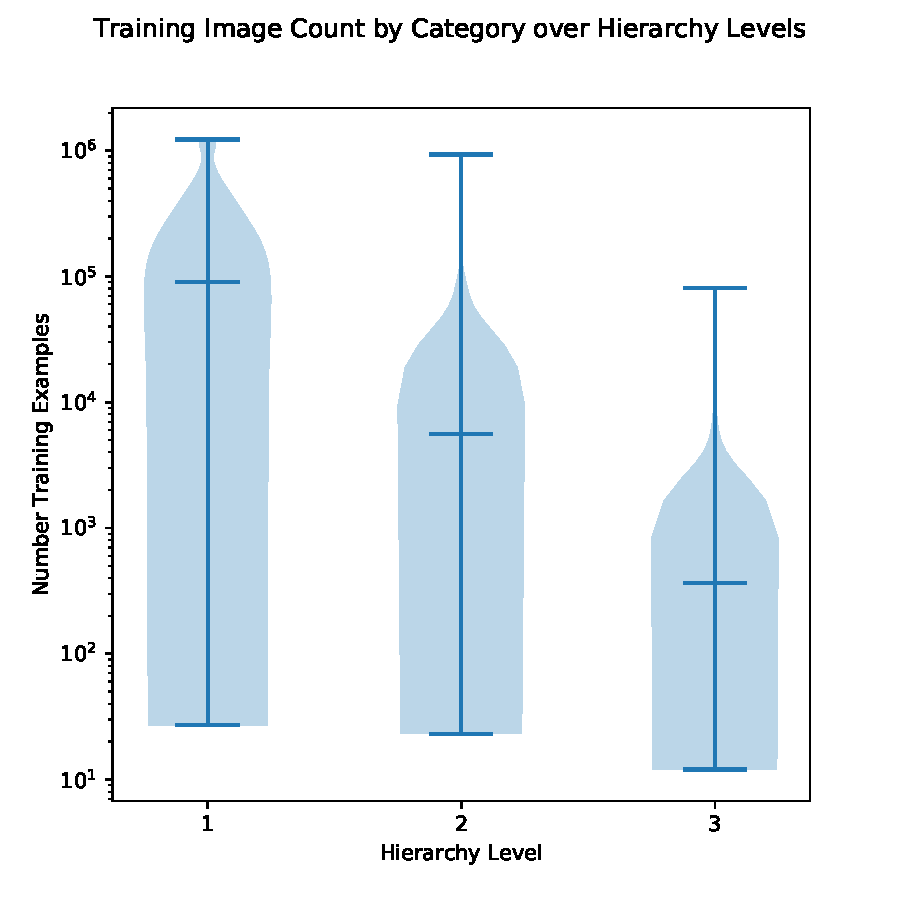
\includegraphics[width=\columnwidth]{img/datacount}
\caption{
This violin plot compares the number of training examples available for first (top) level categorizations, second level categorizations, and third (bottom) level categorizations.
As would be expected, the median training data count is highest for first level categories and lowest for third level categories.
On all three hierarchical levels, training data is distributed unevenly between categories.
For example, although the median top level category has approximately $10^5$ training examples, some have fewer than 100.
In all three subplots, horizontal bars mark the 0, 50, and 100th percentile counts.
}
\label{fig:datacount}
\end{figure}

Cdiscount has made an extensive dataset available through the data science platform Kaggle.
This dataset includes the full hierarchical categorization scheme used by Cdiscount and a listing of over 9 million products.
Each product has a unique ID, the ID of the category it falls in, and one to four images of that product.
The dataset comes divided into training and testing datasets, with the training set describing approximately 7 million products and the testing set describing approximately 2 million products.
Figure \ref{fig:example-images} shows example images from the Cdiscount dataset.
In this dataset, each image has 3 different levels of categorization, making this a challenging multi-classification problem.

Figure \ref{fig:catcount} shows the distribution of category-to-subcategory branching.
Figure \ref{fig:datacount} shows the distribution of availability of training data over all categories in each hierarchy level.
As described in the figure captions, the categorical branching factors and data availabilities vary widely across the dataset.
These irregularities make the Cdiscount challenge more difficult: some categories have many fewer training examples than other categories at the same hierarchy level and some categories have many more subcategories than others.

